% Auto-generated from paper/submission.md by scripts/md_to_latex.py
\documentclass[conference]{IEEEtran}
\usepackage{graphicx}
\usepackage{amsmath,amssymb}
\usepackage{amsthm}
\usepackage{booktabs}
\newtheorem{theorem}{Theorem}
\newtheorem{lemma}{Lemma}
\newtheorem{corollary}{Corollary}
\newtheorem*{theoremstar}{Theorem}
\newtheorem*{lemmastar}{Lemma}
\begin{document}
\title{Exact Budgeted Soft-Information Fusion for UAV-ISAC under Correlated Reporting Losses}
\author{\IEEEauthorblockN{Author Placeholder}\IEEEauthorblockA{Department, University, City, Country}}
\maketitle
\begin{abstract}
Multistatic UAV-ISAC sensing produces correlated soft evidence that must be quantized, transmitted over error-prone reporting links, and selectively fused under a finite bit budget.  We formulate this post-communication chain as a moment-matched Gaussian detection problem whose H0/H1 statistics include quantization, binary-symmetric-channel (BSC) errors, and correlated erasures, and we derive a one-parameter linear fusion family whose KKT-optimal member is the $P_D$-optimal linear score whenever the operating point has $P_D>0.5$.  Set monotonicity is obtained independently as feasible-region nesting, and a bounded-regime submodularity guarantee is stated with explicit conditions.  When variable-rate reporting makes report costs heterogeneous, we replace the equal-cost certificate by an exact multiple-choice knapsack budget selector and an exact worst-target max-min selector, together with a branch-and-bound threshold certificate whose pruning bound is stated and verified.  The framework is instantiated for a UAV-ISAC scenario with a geometry-aware normalized RIS power-gain model, and the numerical audit separately reports combinatorial exactness, value-oracle discretization, and statistical evidence.
\end{abstract}
\begin{IEEEkeywords}
UAV-ISAC, distributed detection, selective fusion, quantized soft information, exact optimization, correlated reporting losses.
\end{IEEEkeywords}
\section{Introduction}
Integrated sensing and communication (ISAC) on UAV platforms must reconcile three tensions: sensing creates correlated per-UAV evidence, reporting links are finite-rate and error-prone, and the sensing and control planes compete for the same resource budget.  Prior UAV-ISAC work emphasizes trajectory, beamforming, and resource allocation \cite{liu2022fundamental}, \cite{meng2024uavisac}, \cite{kumari2018ieee80211ad}; RIS-assisted ISAC optimizes phase profiles or placement \cite{wu2019irs}, \cite{xu2024risisac}, \cite{tun2023risjsac}; distributed detection with quantized soft decisions, sparse sensor selection, and knapsack-style radar sensor selection is well developed \cite{tenney1981detection,chair1986optimal,varshney1997book,nurellari2015quantized}, \cite{chepuri2016sparse,liu2016sensor,guo2022nonparametric,krause2008robust,godrich2012sensor}, but typically under independent observations or a fixed report channel.  The gap addressed here is the selective fusion of post-communication correlated soft evidence under heterogeneous report costs and correlated reporting losses, with exactness certificates for the combinatorial selection layer.
This paper makes three contributions.
\begin{enumerate}
\item A communication-in-the-loop system model in which quantization, BSC errors, detectable erasures, and the random received report set are propagated into H0/H1 evidence moments before fusion, with a concrete correlated-erasure model.
\item A KKT-derived $P_D$-optimal linear fusion family with an independent zero-extension monotonicity argument, an expected-$P_D$ selection objective over the exact reception law, and exact heterogeneous-cost budget/max-min selection certificates with a stated branch-and-bound pruning bound.
\item An audited, reproducible UAV-ISAC application study in which a geometry-aware RIS power-gain model changes the local evidence quality under one normalized report/control budget; multi-seed paired comparisons, two-sided statistics with multiplicity correction, and explicit recording of where guarantees do not apply are included.
\end{enumerate}
The remainder of the paper is organized as follows.  Section 2 reviews the related work.  Section 3 states the system model.  Section 4 derives the method.  Section 5 describes the simulation setup.  Section 6 reports the results.  Section 7 discusses limitations, and Section 8 concludes.
\section{Related Work}
\subsection{UAV-ISAC and DD-domain sensing context}
UAV-ISAC is an active application scenario for correlated multistatic evidence \cite{hadani2017otfs}, \cite{yuan2023ddisac}, \cite{liu2022fundamental}, \cite{meng2024uavisac}.  OTFS concentrates doubly selective channels in the delay-Doppler (DD) domain \cite{hadani2017otfs}, \cite{yuan2023ddisac}, \cite{raviteja2018interference}; any such front end that produces moment-matched Gaussian local evidence can feed the framework proposed here.  We do not claim a new waveform or receiver design, and the selection/fusion theory does not depend on a specific DD-domain model.
\subsection{RIS-assisted ISAC}
RIS creates controllable propagation paths and is a 6G enabler for ISAC \cite{wu2019irs}, \cite{xu2024risisac}, \cite{tun2023risjsac}.  Prior work treats RIS phase as a beamforming variable for waveform or link quality, or jointly allocates radio resources and phase shifts \cite{tun2023risjsac}.  In this paper RIS is an application instance: it changes the per-target evidence moments, and its control overhead competes with report bits under one normalized budget proxy.  It is not a claim about a new RIS beamforming design.
\subsection{UAV-ISAC}
UAVs add mobility and deployment flexibility to ISAC \cite{meng2024uavisac}.  Existing surveys emphasize trajectory, beamforming, and bandwidth, but do not model the selective soft-information reporting chain after quantization, BSC, and correlated erasures.
\subsection{Distributed detection and soft-information fusion}
Distributed detection with quantized soft decisions is a classical problem \cite{tenney1981detection,chair1986optimal,varshney1997book,nurellari2015quantized}.  The likelihood-ratio fusion rule of Chair and Varshney \cite{chair1986optimal} and the person-by-person-optimal local rules of Tenney and Sandell \cite{tenney1981detection} assume independent observations.  Sparse sensor selection has been studied for distributed detection \cite{chepuri2016sparse}, estimation under correlated measurement noise \cite{liu2016sensor}, nonparametric decentralized detection with quantizer design \cite{guo2022nonparametric}, robust submodular observation selection \cite{krause2008robust}, and radar sensor selection as a knapsack problem \cite{godrich2012sensor}.  Exact Poisson-binomial counting \cite{wang1993poisson} and consensus algorithms \cite{olfati2004consensus} certify distributed majority but do not model correlated common-state erasures or set-dependent fusion ranking.  Relative to this literature, our contribution is the combination of a post-communication correlated value model, heterogeneous report costs, and an exact max-min selection certificate, with the conditions for the submodular shortcut stated explicitly.
\subsection{Communication-constrained ISAC resource allocation}
ISAC resource allocation has moved toward joint beamforming/bandwidth/power under sensing constraints \cite{xu2024risisac}, \cite{zargari2024riemannian}, \cite{liu2020joint}, \cite{kumari2018ieee80211ad}, \cite{tun2023risjsac}.  These schemes split time/frequency/power between radar and communication but do not allocate per-report quantization bits and report/control overhead under an expected-$P_D$ objective with an exact combinatorial certificate.
\subsection{Positioning}
We are not aware of prior work that couples the correlated post-communication evidence chain with exact heterogeneous-cost max-min selection certificates under an explicit value oracle and a stated pruning bound.  Distributed majority counting and RIS resource allocation are treated here as secondary application audits, not as claims about a new physical-layer system.
\section{System Model}
\begin{figure}[htbp]
\centering
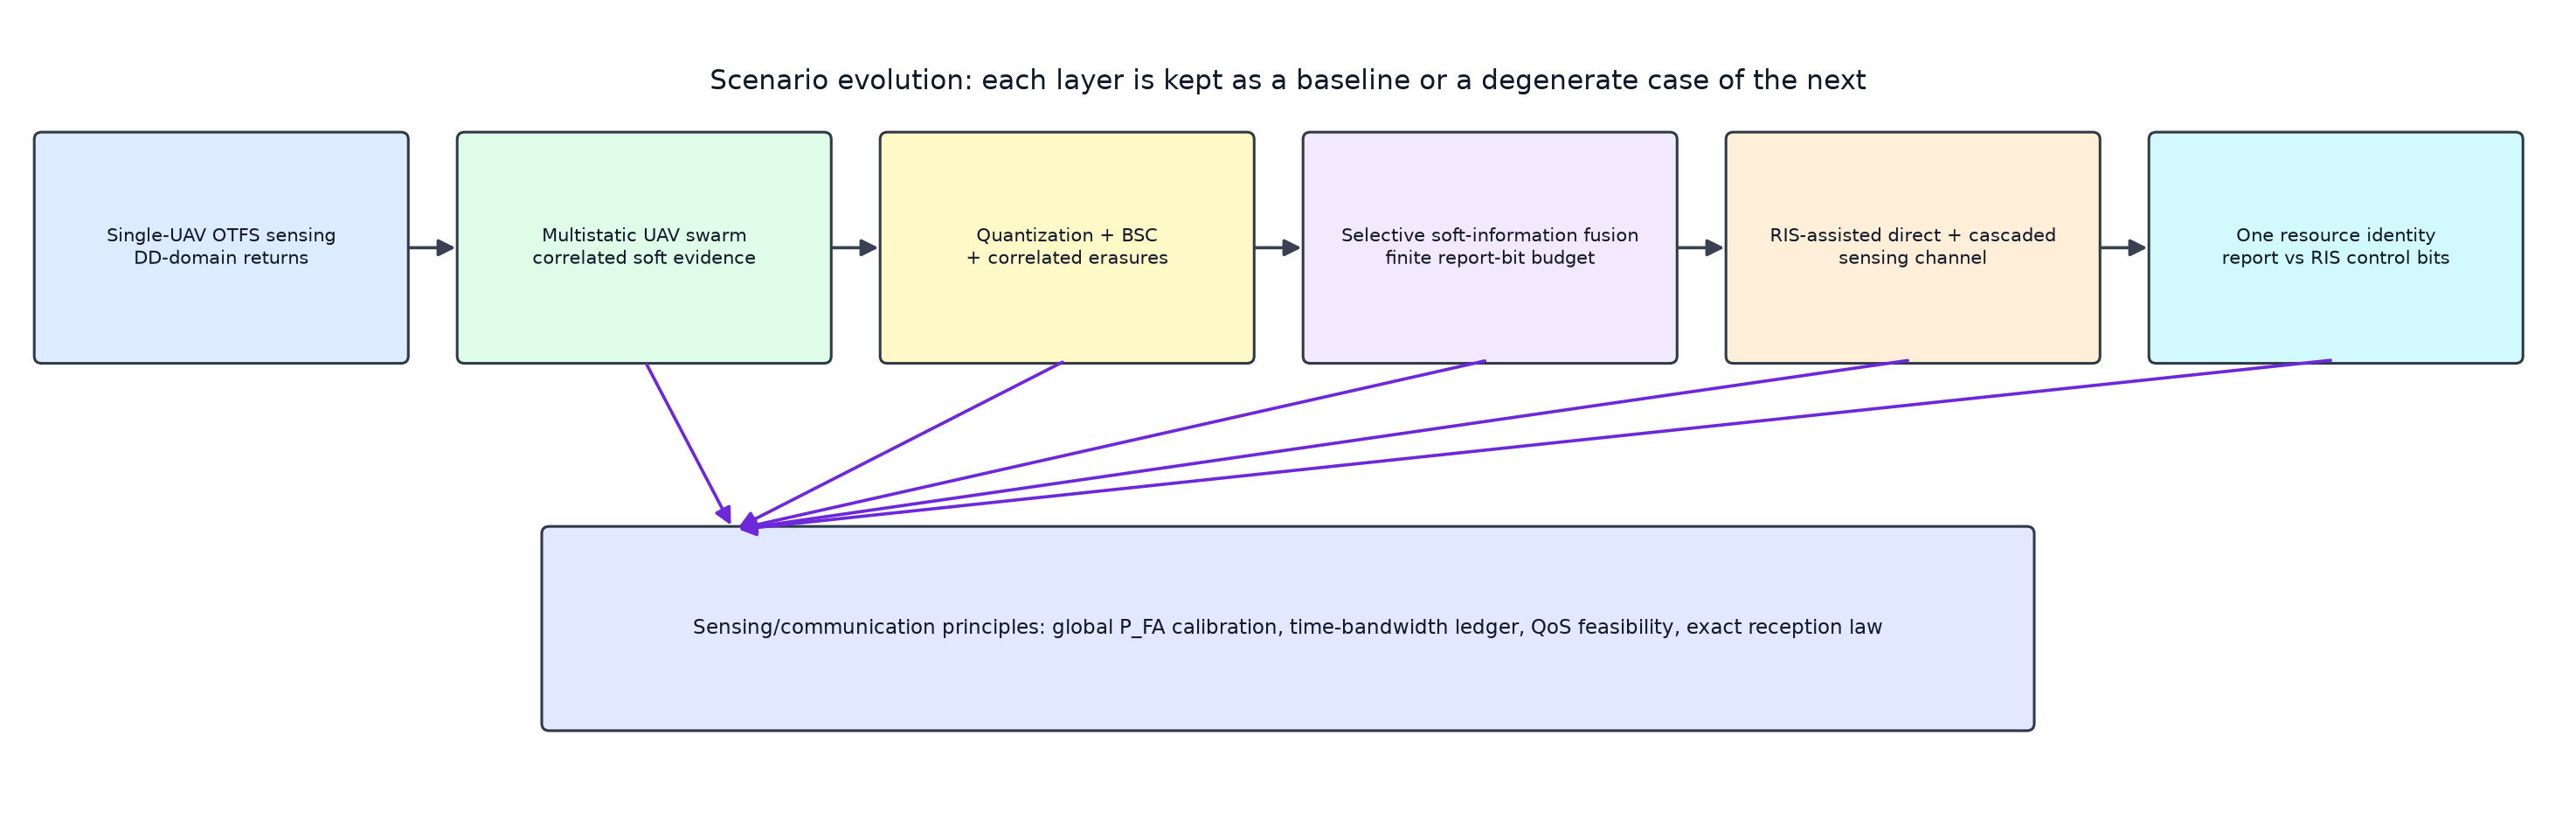
\includegraphics[width=0.92\linewidth]{../paper_figures/scenario_evolution.png}
\caption{Scenario evolution: UAV-ISAC sensing as a source of correlated soft evidence, quantization/BSC/correlated erasures, selective fusion under a finite report-bit budget, and an optional RIS-assisted geometry-aware power-gain instance.}
\end{figure}
\subsection{Evidence and communication chain}
Let $M$ transmitting UAVs serve $Q$ target hypotheses with one receive array.  Per-UAV evidence under H0/H1 is moment-matched Gaussian $(\mu_0,\mu_1,\Sigma_0,\Sigma_1)$ with $\Sigma_0,\Sigma_1\succ 0$.  A report $i$ costs $b_i$ bits and passes through the following chain:
\begin{equation}
\begin{gathered}
X_i \xrightarrow{Q_{b_i}}
\mathbf{c}_i(X_i) \xrightarrow{\text{BSC}}
\tilde{\mathbf{c}}_i \xrightarrow{\text{dequant}}
\hat{X}_i \xrightarrow{\text{erasure mask}}
\gamma_i \hat{X}_i,
\end{gathered}
\end{equation}
where $Q_{b_i}$ is a $b_i$-bit scalar quantizer with thresholds $\tau_{i,1}<\cdots<\tau_{i,2^{b_i}-1}$, reconstruction values $r_i(c)$, and bit labels $c_i(x)\in\{0,1\}^{b_i}$.  The BSC flips each bit independently with probability $\epsilon_i$; dequantization maps the received bit word to $r_i(\tilde{\mathbf{c}}_i)$.  Erasure is modeled by $\gamma_i\in\{0,1\}$; erased reports are omitted from fusion.
The erasure mask is correlated across UAVs through a common block state $Z\in\{0,1\}$ and independent per-link success events $V_i\sim\mathrm{Bernoulli}(s_i)$:
\begin{equation}
\begin{gathered}
\gamma_i = Z V_i,
\qquad
\Pr(\gamma)=\begin{cases}
1-p_z, & \gamma=\mathbf{0},\\
p_z \prod_i s_i^{\gamma_i}(1-s_i)^{1-\gamma_i}, & \gamma\neq\mathbf{0}.
\end{cases}
\end{gathered}
\end{equation}
This is the concrete correlated-communication-loss model referenced by the title.  Conditional on the reception pattern $\gamma$, the fused observation is the subvector of reconstructed reports with $\gamma_i=1$. Its conditional moments are
\begin{equation}
\begin{gathered}
\mu_h^{(\gamma)} =
\mathbb{E}[\hat{\mathbf{X}}_\gamma \mid H_h,\gamma],
\qquad
\Sigma_h^{(\gamma)} =
\operatorname{Cov}[\hat{\mathbf{X}}_\gamma \mid H_h,\gamma],
\end{gathered}
\end{equation}
which are obtained by propagating the quantizer cells, the BSC transition probabilities, and the dequantization map through the moment-matched Gaussian distribution.  For example, the conditional mean of a received report is
\begin{equation}
\begin{gathered}
\mathbb{E}[\hat{X}_i\mid H_h,\gamma_i=1]
= \sum_{c\in\{0,1\}^{b_i}} r_i(c)\,
\Pr(\tilde{\mathbf{c}}_i=c\mid H_h),
\end{gathered}
\end{equation}
with the BSC transition matrix $\Pr(\tilde{\mathbf{c}}=c'\mid \mathbf{c}=c)= \epsilon_i^{d_H(c,c')}(1-\epsilon_i)^{b_i-d_H(c,c')}$. The fusion threshold is recomputed from the received-set moments, so $P_{FA}$ is calibrated per reception pattern rather than for the nominal all-received set.  The primary metrics are mean and worst-target expected $P_D$ over the erasure law $\Pr(\gamma)$.
\subsection{Fusion and resource identity}
The linear fusion score is $s = w^\top x$ with threshold $\tau = w^\top \mu_0 + z\sqrt{w^\top\Sigma_0 w}$, where $z = \Phi^{-1}(1-P_{FA})$.  The detection probability is
\begin{equation}
\begin{gathered}
P_D(w) = \Phi\!\left(
\frac{w^\top\delta - z\sqrt{w^\top\Sigma_0 w}}
{\sqrt{w^\top\Sigma_1 w}}
\right),
\end{gathered}
\end{equation}
with $\delta = \mu_1-\mu_0$.  The RIS application model changes the effective evidence gain $g_{iq}$ of report $i$ for target $q$.  The controlled model is $g_{iq} = 1 + (\mathrm{strength}_q\, \mathrm{array_gain}_{iq})^2$; the geometry-aware normalized power-gain model uses
\begin{equation}
\begin{gathered}
P_{\mathrm{dir}} = \frac{1}{R_{tx}^2 R_{rx}^2},
\qquad
P_{\mathrm{ris}} =
\frac{N_{\mathrm{ris}}^2\,\mathrm{array_gain}_{iq}^2\,
a_{\mathrm{ap}}}
{R_1^2 R_2^2 R_3^2},
\end{gathered}
\end{equation}
and $g_{iq} = 1 + P_{\mathrm{ris}}/P_{\mathrm{dir}}$, with an optional direct-path blockage factor for the weak target.  This is a normalized power-gain proxy: in general the direct and RIS paths should be added as complex amplitudes,
\begin{equation}
\begin{gathered}
P_{\mathrm{tot}} = \left|
\sqrt{P_{\mathrm{dir}}}\,e^{j\phi_d} +
\sqrt{P_{\mathrm{ris}}}\,e^{j\phi_r}
\right|^2,
\end{gathered}
\end{equation}
so the coherent cross term $2\sqrt{P_{\mathrm{dir}}P_{\mathrm{ris}}} \cos(\phi_r-\phi_d)$ can be negative.  The power-additive form is therefore an approximation valid when the two paths are separable in the DD domain, or when $\phi_r$ is aligned to $\phi_d$; we do not claim that an uncontrolled RIS phase never reduces a link's evidence SNR.
The control/report resource identity is
\begin{equation}
\begin{gathered}
B_{\mathrm{total}} =
B_{\mathrm{report}} +
N_{\mathrm{ris}}\cdot\frac{b_{\mathrm{phase}}}{C},
\end{gathered}
\end{equation}
where $C$ is the coherence-frame count.  This is a normalized budget proxy, not a true time-bandwidth identity: channel coding, headers, control-plane signaling, RIS estimation, and retransmission overhead are not modeled. Under the conservative one-symbol-per-bit convention, report and control bits map to time-bandwidth symbols.
\begin{table}[htbp]
\centering
\resizebox{\linewidth}{!}{
\begin{tabular}{ll}
\toprule
Symbol & Meaning \\
\midrule
$M$, $Q$ & UAV count, target count \\
$\mu_0,\mu_1,\Sigma_0,\Sigma_1$ & H0/H1 evidence moments \\
$b_i$ & bit cost of report $i$ \\
$\epsilon_i$ & BSC bit-flip probability of report $i$ \\
$P_{FA}$, $P_D$ & false-alarm and detection probabilities \\
$B_{\mathrm{total}}$, $B_{\mathrm{report}}$ & total and report budgets \\
$N_{\mathrm{ris}}$, $b_{\mathrm{phase}}$, $C$ & RIS elements, phase bits, coherence frames \\
$S_q$ & report schedule of target $q$ \\
$m_q(t)$ & minimum bit cost for target $q$ to reach threshold $t$ \\
$L_{\min}$ & exact first-feasible majority prefix length \\
\bottomrule
\end{tabular}
}
\caption{Notation.}
\end{table}
Abbreviations: ISAC (integrated sensing and communication), UAV (unmanned aerial vehicle), RIS (reconfigurable intelligent surface), BSC (binary symmetric channel), DD (delay-Doppler), QoS (quality of service), KKT (Karush-Kuhn-Tucker), DP (dynamic programming).
\section{Method}
Figure 2 shows how the proposed chain evolves from classical distributed detection to exact selective fusion.  Each stage keeps the prior element as a baseline or a degenerate case, so the experimental gates audit the transition between adjacent stages.
\begin{figure}[htbp]
\centering
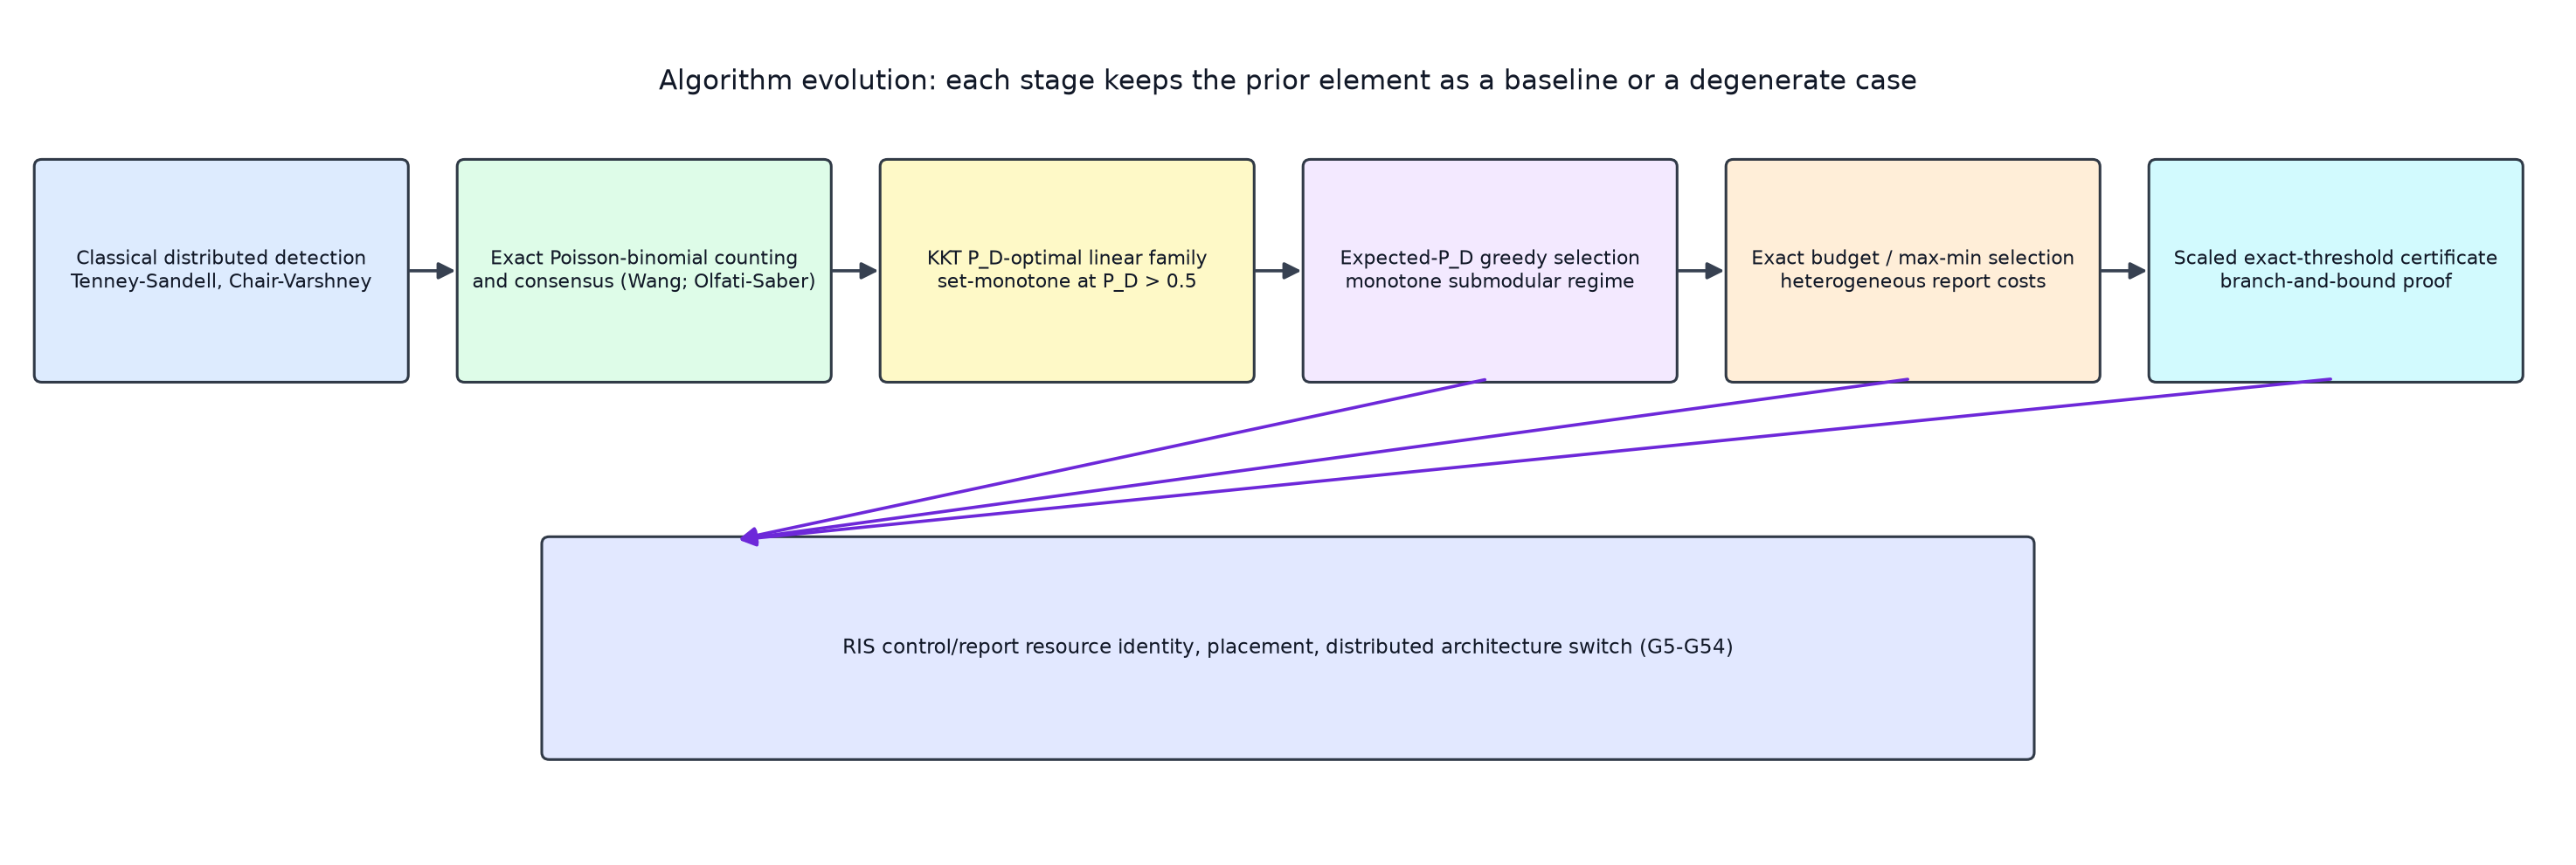
\includegraphics[width=0.92\linewidth]{../paper_figures/algorithm_evolution.png}
\caption{Algorithm evolution: person-by-person optimal local rules and likelihood-ratio fusion, exact Poisson-binomial counting and consensus, KKT $P_D$-optimal fusion, expected-$P_D$ greedy selection, exact heterogeneous-cost budget/max-min selection, scaled threshold certificate, and the RIS/control-budget and distributed architecture layers.}
\end{figure}
\subsection{$P_D$-optimal linear fusion}
Let $\Sigma_0=LL^\top$ with $L$ invertible, and use the whitened coordinates $y=L^\top w$, $a=L^{-1}\delta$, $Q=L^{-1}\Sigma_1 L^{-\top}$.  The detection probability is
\begin{equation}
\begin{gathered}
P_D = \Phi\!\left(
\frac{a^\top y - z\|y\|}{\sqrt{y^\top Q y}}
\right).
\end{gathered}
\end{equation}
Maximizing $P_D$ is equivalent to maximizing $F(y)=a^\top y-z\|y\|$ over the compact ellipsoid $y^\top Q y=1$.  The objective is scale-invariant in $y$, so the ellipsoid normalization fixes the scale without loss of generality.  At a stationary point,
\begin{equation}
\begin{gathered}
a - z\frac{y}{\|y\|} - 2\lambda Q y = 0.
\end{gathered}
\end{equation}
Left-multiplying by $y^\top$ and using $y^\top Q y=1$ gives
\begin{equation}
\begin{gathered}
2\lambda = a^\top y - z\|y\| = F(y).
\end{gathered}
\end{equation}
If $P_D>0.5$, then $F(y)>0$ and hence $\lambda>0$.  The stationarity condition therefore yields
\begin{equation}
\begin{gathered}
y \propto (Q+\mu I)^{-1} a,
\qquad
\mu = \frac{z}{2\lambda\|y\|}\ge 0,
\end{gathered}
\end{equation}
so any global optimum direction lies in the one-parameter family $w(\mu)=L^{-\top}(Q+\mu I)^{-1}L^{-1}\delta$.  The endpoints $\mu=0$ and $\mu\to\infty$ are included in the search (the latter as the deflection limit), and the one-dimensional search is performed over a dense grid with a controlled tolerance.  Consequently, when every candidate subset has an optimal operating point with $P_D>0.5$, optimizing the one-parameter family attains the global linear optimum.
\begin{lemma}[zero-extension monotonicity]
Let $S\subseteq T$ and let the
moments on $S$ be the consistent principal submatrix of the moments on $T$.
Taking the optimal weights of $S$ and zero-extending them to $T$ preserves
the score and hence preserves $P_D$, so
$P_D^\star(T)\ge P_D^\star(S)$.  This is feasible-region nesting, independent
of the KKT parametrization.
\end{lemma}
In the proportional regime $\Sigma_1=c\Sigma_0$, the family degenerates to
\begin{equation}
\begin{gathered}
P_D = \Phi\!\left(
\frac{\sqrt{D(S)}-z}{\sqrt{c}}
\right),
\qquad
D(S) = \delta_S^\top \Sigma_{0,SS}^{-1}\delta_S.
\end{gathered}
\end{equation}
This closed form is used in Section 4.2 to state the submodularity boundary.
\subsection{Expected-$P_D$ selection}
For target $q$ and schedule $S_q$, the objective is
\begin{equation}
\begin{gathered}
\mathbb{E}_{P_D}(q,S_q) =
\mathbb{E}_{\gamma}\big[
P_D\big(\mathrm{owner}\cup \mathrm{received}(S_q,\gamma)\big)
\big].
\end{gathered}
\end{equation}
The two-stage greedy first minimizes the normalized miss-deficit and then maximizes expected-$P_D$ gain per report bit.  Every fixed-pattern $P_D$ is set-monotone at the audited operating points, so the expectation is monotone.
In the proportional regime, set $x=\sqrt{D}$.  The map $P_D(D)=\Phi((x-z)/\sqrt{c})$ is concave in $D$ if and only if
\begin{equation}
\begin{gathered}
x^2 - z x + c \ge 0.
\end{gathered}
\end{equation}
Consequently:
\begin{itemize}
\item If $c\ge z^2/4$, concavity holds for every $D>0$.
\item Otherwise, concavity holds in the strong-evidence region
\end{itemize}
$x\ge (z+\sqrt{z^2-4c})/2$, i.e. $\sqrt{D}\ge (z+\sqrt{z^2-4c})/2$, and also in a low-evidence interval; the strong-evidence threshold is the one used by the audit.
The modularity of the deflection $D(S)$ requires a diagonal $\Sigma_0$: then $D(S)=\sum_{i\in S}\delta_i^2/\sigma_{0,i}^2$ is additive. For general correlated $\Sigma_0$, $D(S)=\delta_S^\top\Sigma_{0,SS}^{-1}\delta_S$ is not modular and need not be submodular.  In addition, the erasure law $\Pr(\gamma)$ must not be coupled to the chosen schedule; if scheduling changes the erasure distribution, the expectation of a set-submodular function is not necessarily submodular.  Under proportional covariance, diagonal $\Sigma_0$, the strong-evidence condition above, and schedule-independent erasures, the expected objective is monotone submodular and equal-cost cardinality greedy inherits the classical $1-1/e$ bound.  The implemented bit-budgeted greedy does not inherit that ratio and is not claimed to.
\subsection{Exact selection under heterogeneous report costs}
Variable-rate reporting makes per-report costs heterogeneous, so the equal-cost quota certificate no longer covers the feasible set.  Let $\mathcal{O}_q$ be the set of all $(\mathrm{cost}(S),P_D(S))$ pairs obtained by enumerating every subset of non-owner reports for target $q$.  A global schedule chooses one option per target with total cost at most $B$.  This is a multiple-choice knapsack, solved by a dynamic program over targets and accumulated bits in which states are pruned only by componentwise Pareto dominance.
\begin{theorem}[exactness of the budget DP]
Under additive report costs and
target-separable report option sets with no cross-target coupling, for every
target enumerate all report subsets and their exact bit costs.  For any two
partial schedules with the same accumulated cost, if one has $P_D$ no
smaller in every processed target, then every monotone completion of the
dominated schedule is no better than the corresponding completion of the
dominating one.  Keeping only componentwise-Pareto value vectors preserves
at least one optimal path, so the DP terminates with the exact lexicographic
optimum $(QoS\ gap,\ weighted\ mean,\ worst\ target)$.
\end{theorem}
The system-level objective is worst-target expected $P_D$.  For a threshold $t$, feasibility asks whether each target can choose a subset with value at least $t$ under the total budget; this is again a multiple-choice knapsack feasibility problem.  Because feasibility is monotone in $t$, the exact max-min value is found by binary search over the finite set of per-target subset values, and the returned schedule is feasible at the optimal threshold.
\begin{theorem}[exact max-min selection]
Under the same target-separable,
additive-cost assumptions, let
$\mathcal{T}=\{t_1<\cdots<t_K\}$ be the finite set of enumerated per-target
subset values.  The threshold-feasibility DP returns a feasible schedule
with $\min_q P_D(q,S_q)=\max_{t\in\mathcal{T}}\{t : \text{feasible}(t)\}$,
and among schedules attaining that threshold it returns the lexicographically
best secondary score.
\end{theorem}
\begin{corollary}[joint bit allocation and selection]
Under the same
target-separable, additive-cost assumptions, replace each report option by
the mutually exclusive options $\{$not selected, 1-4 bit quantized$\}$ with
their post-communication moments and bit costs.  The option set remains
finite and target-separable, so Theorem 1 and Theorem 2 hold unchanged: the
exact DP returns the global joint optimum over report selection and
per-report quantization bits, with no concavity or diminishing-returns
assumption.
\end{corollary}
\subsection{Scaled exact-threshold certificate}
For larger report sets, define $m_q(t)$ as the minimum bit cost for target $q$ to reach $t$.  A global schedule with all values at least $t$ exists if and only if $\sum_q m_q(t)\le B$, because the per-target minima are jointly attainable and every feasible subset costs at least its minimum.
\begin{theorem}[exact minimum-cost certificate]
Let $m_q(t)$ be computed by
branch-and-bound with the dual Cauchy upper bound.  In whitened coordinates
for a candidate set $S$, let $\lambda_{\min},\lambda_{\max}$ be the extreme
eigenvalues of $Q_S$ and define
\end{theorem}
\begin{equation}
\begin{gathered}
A_S(\mu)=\sqrt{a_S^\top(Q_S+\mu I)^{-1}a_S},
\qquad
\mu\ge 0.
\end{gathered}
\end{equation}
Then every linear score satisfies
\begin{equation}
\begin{gathered}
s(y) \le \min_{\mu\ge 0}\ \max\Bigl\{
\\
A_S(\mu)\sqrt{1+\mu/\lambda_{\max}} - z/\sqrt{\lambda_{\max}},\\
A_S(\mu)\sqrt{1+\mu/\lambda_{\min}} - z/\sqrt{\lambda_{\min}}
\Bigr\}.
\end{gathered}
\end{equation}
For any $\mu\ge 0$, Cauchy-Schwarz with the factor $(Q_S+\mu I)^{1/2}$ gives $a_S^\top y\le A_S(\mu)\sqrt{y^\top(Q_S+\mu I)y}= A_S(\mu)\sqrt{1+\mu\|y\|^2}$, and Rayleigh's quotient gives $\|y\|\in[1/\sqrt{\lambda_{\max}},1/\sqrt{\lambda_{\min}}]$.  The majorant $g(t)=A_S(\mu)\sqrt{1+\mu t^2}-zt$ is convex in $t$, so its maximum on the interval is attained at an endpoint; minimizing over $\mu$ keeps the bound valid and no tighter than the $\mu=0$ Cauchy bound $\sqrt{a_S^\top Q_S^{-1}a_S}-z/\sqrt{\lambda_{\max}}$ (with $\lambda_{\min}$ when $z<0$).  When remaining reports are added, the enlarged covariance is a principal extension and the bound is recomputed on the union set, so no Schur-complement error is introduced.  A node is pruned only when that bound is below $t$, when its cost already reaches the best known cost, or when the cheapest remaining reports cannot beat the best known cost.  The returned cost is therefore the exact minimum, and pruning never changes the result.  The implementation uses a value cache, a 33-point $\mu$ grid with local refinement, and an explicit tolerance of $10^{-12}$ on the threshold comparison, so the claim is exact with respect to the tolerance-controlled value oracle.
Small low-$P_D$ models use exact subset enumeration instead; when every model is within \texttt{max\_exhaustive\_reports}, the scaled selector delegates directly to the exact selector rather than running an epsilon binary search. The worst case remains exponential, and the bound is reported as a pruning certificate, not a polynomial-time guarantee.
\subsection{Complexity}
The exact budget DP processes $Q$ targets, $B$ cost states, and a per-target cost-value Pareto option set whose size is at most the number of distinct subset costs.  Its complexity is $O(Q \cdot B \cdot |\mathcal{F}| \cdot S)$ with state-pruning factor $S$; componentwise dominance removes options that are no cheaper and no better, so in the audited models the option set is the cost-value frontier rather than the full exponential subset list.  The max-min selector adds a binary search over the finite candidate threshold set, multiplying the DP by $O(\log K)$ feasibility checks.  G8-S keeps the same threshold search but replaces per-target subset enumeration by branch-and-bound; its worst case is exponential, while the greedy warm start and cost-bounded minimality proof make the audited 24-report instance finish in 35 ms.  The exact majority certificate evaluates Poisson-binomial tails by a $O(N^2)$-state DP over the voter prefix when decisions are independent conditional on the hypothesis; when independence holds only after conditioning on a common state, the mixture form is used instead.  It does not rely on the Gaussian approximation or on monotonicity of feasibility in the prefix length.
\subsection{Application instance: geometry-aware RIS power gain}
The RIS application model uses a target-aligned beam codebook with $b$-bit uniform phase quantization.  The mean array-gain loss is $\mathrm{sinc}^2(1/2^b)$ in the large-$N$ limit, with the finite-$N$ correction $1/N+(1-1/N)\mathrm{sinc}^2(1/2^b)$.  Placement and phase-bits are searched over a finite candidate set in the application audit only. These searches use coarse-to-fine refinement with an $L$-Lipschitz grid loss bound $Lh\sqrt{d}/2$; they are not part of the core selection/fusion theory and do not claim physical-layer optimality.
\subsection{Exact first-feasible majority prefix}
For the distributed branch, local 1-bit decisions with probabilities $p_{0,i},p_{1,i}$ are fused by a counting rule.  The exact type-I/II probabilities are Poisson-binomial tails only when the decisions are independent conditional on the hypothesis.  If only conditional independence given a common state $Z$ holds, the exact tail is $\mathbb{E}_Z[P_{\mathrm{PB}}(k;p_{h,i}(Z))]$ rather than a single Poisson-binomial tail.  The certificate below returns the first feasible prefix of a fixed voter sequence; it is not a global minimum over arbitrary voter subsets.
\begin{theorem}[exact first-feasible prefix]
For a fixed voter sequence,
\texttt{exact\_min\_majority\_uavs} evaluates the exact tail on every prefix and
returns the first feasible prefix.  Feasibility is not monotone in the
prefix length in general; the audit exhibits sequences with trace
$[F,F,T,F,T]$.  Consequently binary search over the prefix length is valid
only when the per-sequence monotonicity certificate is available.
\end{theorem}
\section{Simulation Setup}
The audited demo configuration uses $M=8$ UAVs and $Q=3$ targets with the same false-alarm rate and QoS weighting as the repository's \texttt{demo.yaml}. Report budgets are swept over $\{3,5,7,9,11\}$ bits for the exact selection audits and over total budgets $\{20,28,40\}$ for the RIS/architecture audits.  The exact selection experiments use 500 seeds and a 64-point expectation grid; the RIS/architecture experiments use 4-12 seeds and 512-point grids as documented in the audit.  A separate target-count scalability audit uses 3 seeds and a 32-point grid at $Q=3/4/5$.  Every number reported below is mean over seeds unless stated otherwise.  The full result table is \texttt{../results/paper\_results\_table.md}.
The term "exact" in this paper has three levels.  The combinatorial DP and branch-and-bound results are exact with respect to a given per-subset value oracle; the oracle itself uses a finite expectation grid (64 or 512 points) and a one-dimensional $\mu$ search with a controlled tolerance.  We therefore claim combinatorial exactness given the discretized / tolerance-controlled value oracle, not end-to-end exactness of the continuous expectation.
\begin{table}[htbp]
\centering
\resizebox{\linewidth}{!}{
\begin{tabular}{ll}
\toprule
Parameter & Value \\
\midrule
UAVs $M$ & 8 \\
Targets $Q$ & 3 \\
False-alarm rate $P_{FA}$ & 0.05 \\
Nominal quantizer bits per report & 3 \\
Default report budget $B_{\mathrm{report}}$ & 42 bits \\
DD-domain Doppler bins / delay bins / accumulation & 16 / 32 / 8 \\
UAV SNR range & -7 to 5 dB \\
Fractional Doppler range & $[-0.48,0.48]$ \\
Residual DD-domain interference & 0.12 \\
Common correlation factor & 0.30 \\
Report success probability range & $[0.72,0.98]$ \\
BSC bit-flip range & $[0.005,0.08]$ \\
Exact-selection audit & 500 seeds, grid 64, $B\in\{3,5,7,9,11\}$ \\
RIS/architecture audit & 4-12 seeds, grid 512, $B\in\{20,28,40\}$ \\
\bottomrule
\end{tabular}
}
\caption{Simulation parameters.}
\end{table}
\subsection{Reproducibility}
All reported numbers are generated by the repository scripts and stored in \texttt{../results/}.  The exact-selection tables are reproduced by
{\footnotesize
\begin{verbatim}
python scripts/run_exact_budget_gate.py --seeds 20 --budgets 3 5 7 9 11 --grid 64
python scripts/run_exact_maxmin_gate.py --seeds 500 --budgets 3 5 7 9 11 --grid 64
python scripts/run_scaled_maxmin_gate.py --seeds 20 --budgets 5 9 --grid 64
python scripts/run_exact_selection_target_scalability.py `
  --seeds 3 --budgets 8 12 16 --grid 32
python scripts/run_scaled_difficulty_gate.py --grid 96
python scripts/audit_exact_selection_stats.py
\end{verbatim}
}
The unified result table and all paper figures are rebuilt by
{\footnotesize
\begin{verbatim}
python scripts/build_paper_tables.py
python scripts/draw_algorithm_evolution.py
python scripts/draw_scenario_evolution.py
python scripts/verify_paper_numbers.py
\end{verbatim}
}
\section{Results}
\subsection{Fusion and selection}
On 1318 operating-point addition edges, the $P_D$-optimal family has zero decreasing edges, while the deflection-optimal score decreases on 258 edges (19.6\%) with a maximum 16.1 pp drop.  The mean gain over the deflection score is +0.63 pp and the maximum per-edge gain is +21.2 pp.
At $B=20$ under correlated erasures, the expected-$P_D$ greedy improves mean expected $P_D$ by +1.14 pp (bootstrap CI $[0.47,1.74]$, 85\% win) and worst-target $P_D$ by +7.56 pp; a two-candidate hybrid gives +1.44 pp mean and +6.50 pp worst-target.  At $B=40$ the greedy alone is -0.91 pp in mean, so the audited claim uses the hybrid and does not claim universal dominance.
The exact-selection audit below uses 20 paired seeds.  The exact budget selector (G8-K) matches the exhaustive global oracle in 100\% of controlled cells and never loses to greedy on the lexicographic score.  The exact max-min selector (G8-M) is never worse than greedy in any audited cell; this is a correctness property of the optimizer, not a statistical discovery. At the system level with variable-rate reporting, the worst-target gains are small in absolute terms (0.20-3.02 pp) but are all significant after a two-sided paired t-test with Holm correction over the five budgets (Holm p=1.0e-7 to 9.7e-47; paired Wilcoxon p<=2.6e-6).  In the constrained oracle scenario, where every target has the same report pool and cost structure, the gains are larger (0.47-6.61 pp at $B=5/7/9/11$) and remain significant after Holm correction.  The 20-seed audit reported in the first revision therefore understated the evidence; the 500-seed audit establishes the max-min layer statistically at every budget point.
\begin{table}[htbp]
\centering
\resizebox{\linewidth}{!}{
\begin{tabular}{ccccc}
\toprule
Budget & G8-M gain (pp) & Two-sided t p & Holm p & Wilcoxon p \\
\midrule
3 & +0.20 & 1.0e-7 & 1.0e-7 & 2.6e-6 \\
5 & +0.94 & 5.3e-13 & 1.1e-12 & 8.5e-19 \\
7 & +2.40 & 4.1e-40 & 1.7e-39 & 9.6e-44 \\
9 & +1.46 & 4.2e-19 & 1.3e-18 & 9.0e-21 \\
11 & +3.02 & 1.9e-47 & 9.7e-47 & 2.4e-47 \\
\bottomrule
\end{tabular}
}
\caption{Exact max-min versus forward greedy (500 seeds, grid 64, system-level variable-rate audit).}
\end{table}
The scaled certificate (G8-S) matches exact selection to zero absolute error on the 500-seed set.  A report-count benchmark covers $R=8/12/16/20/24/28/32/40$ non-owner reports: exhaustive subset counts grow to $2^{24}=16{,}777{,}216$, $2^{32}\approx 4.3\times 10^9$, and $2^{40}\approx 1.1\times 10^{12}$, while the branch-and-bound certificate finishes in 24-60 ms and returns the exact minimum cost (1-2 bits) at every scale.  A difficulty sweep on 10-report models adds critical-threshold, similar-weak, and K-report layers: thresholds $0.75$-$0.90$ require $4$-$9$ reports, the branch-and-bound visits 484-8185 nodes with a recursion depth of 10 and a 50\% prune rate, and every returned minimum matches exhaustive enumeration on all ten audited cells.  A correlated-redundant instance with inter-report correlation 0.95 visits 113 nodes and triggers 15 upper-bound cuts with the dual bound, versus 1791 nodes with the $\mu=0$ Cauchy member, confirming that the parameterized bound becomes active and tight when the remaining reports are highly correlated and hence carry little new evidence.
The target-count audit re-verifies the exhaustive-oracle match when the number of targets grows.  At $Q=3/4/5$ and $B=8/12/16$ (3 seeds each), the budget and max-min selectors match their exhaustive oracles in 100\% of all 27 cells and are never worse than forward greedy.  Mean wall time grows from about 180 ms at $Q=3$ to about 300-360 ms at $Q=5$ (grid 32), so the exactness certificate remains practical at larger target counts.
\begin{table}[htbp]
\centering
\resizebox{\linewidth}{!}{
\begin{tabular}{cccccc}
\toprule
Targets $Q$ & Budget $B$ & Budget wall (ms) & Max-min wall (ms) & Oracle match & Never worse \\
\midrule
3 & 8 & 182 & 176 & 100\% & 100\% \\
3 & 12 & 180 & 184 & 100\% & 100\% \\
3 & 16 & 183 & 175 & 100\% & 100\% \\
4 & 8 & 228 & 234 & 100\% & 100\% \\
4 & 12 & 243 & 237 & 100\% & 100\% \\
4 & 16 & 245 & 241 & 100\% & 100\% \\
5 & 8 & 300 & 302 & 100\% & 100\% \\
5 & 12 & 322 & 312 & 100\% & 100\% \\
5 & 16 & 363 & 351 & 100\% & 100\% \\
\bottomrule
\end{tabular}
}
\caption{Target-count scalability (3 seeds, grid 32).}
\end{table}
Figure 3 shows the max-min wall time as a function of $Q$ for each budget.
\begin{figure}[htbp]
\centering
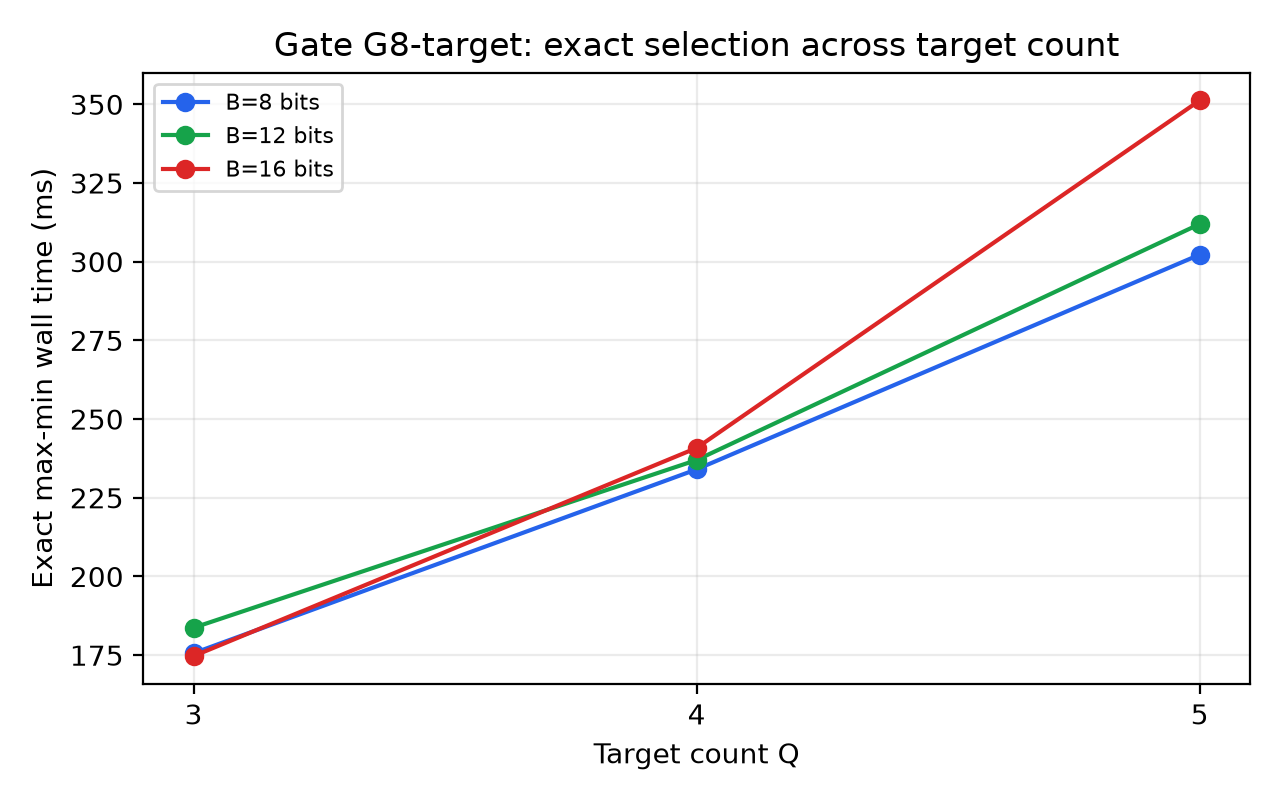
\includegraphics[width=0.92\linewidth]{../paper_figures/g8_target_scalability.png}
\caption{Exact max-min wall time versus target count at report budgets $B=8/12/16$; all cells match the exhaustive oracle and never lose to greedy.}
\end{figure}
\subsection{Application audit: RIS-assisted evidence quality}
At $B=20$, aligned RIS plus expected-$P_D$ greedy gives +12.3 pp mean and +17.8 pp worst-target expected $P_D$ over no RIS, with QoS feasibility rising from 0\% to 95\%.  With the physics-based channel, 1024 elements and aperture scale $10^{-2}$ raise mean and worst-target expected $P_D$ by +16.3 pp and +24.8 pp at $B=20$.  At total budget 40, a jointly optimized 3-bit RIS with 256 elements raises worst-target expected $P_D$ by up to +9.85 pp over a fixed RIS deployment and +19.5 pp over no RIS while using slightly less time-bandwidth.
These numbers illustrate how the fusion/selection layer consumes improved local evidence under the geometry-aware power-gain model.  Subarray multi-beam partitioning, aperture scaling, and array-factor allocation are heuristic extensions outside the exactness theorems; we do not interpret them as physical-layer optimality statements.
\subsection{Extension audit: distributed branch and exact majority}
The distributed-branch and rate-profile consistency audits are collected in Appendix B.  They are extension checks outside the core fusion/selection theory: they verify the exact first-feasible prefix certificate, the correlated-mixture semantics, and the difference between greedy and exact rate-profile optimality, and are not used as standalone contributions.
\subsection{Factorial ablation}
To separate the contribution sources, we toggle one factor at a time at $B=20$ with 500 paired scenarios (Table 5).  Removing the RIS power-gain instance is by far the largest effect: worst-target $P_D$ drops by 22.3 pp and QoS feasibility falls from 100\% to 0.4\%.  The clean-channel upper bound is next (+0.84 pp), followed by $P_D$-optimal fusion (+0.42 pp) and exact max-min selection (+0.13 pp).  Greedy and lexicographic budget schedules coincide on this geometry, so the max-min gain is the worst-target-aware tie-break rather than a different schedule family.  Quantization is assessed separately in Section 6.5 because the strong-evidence demo geometry is not the regime where variable-rate reporting helps.
\begin{table}[htbp]
\centering
\resizebox{\linewidth}{!}{
\begin{tabular}{lcccc}
\toprule
Factor & Worst $P_D$ & Mean $P_D$ & Worst loss vs full (pp) & QoS rate \\
\midrule
Full chain & 0.978 & 0.988 & 0.00 & 100\% \\
Deflection fusion & 0.974 & 0.985 & +0.42 & 100\% \\
Forward greedy & 0.977 & 0.989 & +0.13 & 100\% \\
No RIS & 0.755 & 0.832 & +22.32 & 0.4\% \\
Clean channel & 0.986 & 0.992 & -0.84 & 100\% \\
Lexicographic budget & 0.977 & 0.989 & +0.13 & 100\% \\
\bottomrule
\end{tabular}
}
\caption{Factorial ablation (500 seeds, grid 64, $B=20$).}
\end{table}
The small demo-level max-min gain is a scenario property, not an algorithmic ceiling.  In a hard two-target scenario with one strong target and one weak target whose reports are similar and heterogeneously priced, exact max-min exceeds forward greedy by 2.45-3.26 pp and the lexicographic budget selector by 3.26-3.45 pp at $B=8/10$ over 20 seeds, while both baselines sometimes spend the whole budget on the strong target.
\subsection{Quantization study: variable-rate under a tight budget}
The quantization comparison uses budgets set by the all-report costs: the 1-4 bit variable-rate arm needs 20 bits to schedule all eight reports, while the fixed 3-bit arm needs 24 bits.  Over 10 seeds, variable-rate reporting exceeds fixed 3-bit reporting by 0.80 pp at $B=18$ and by 3.05 pp at $B=20$, with worst-target $P_D$ of 0.910 and 0.932 respectively (Table 6).  At $B=20$ the fixed-rate arm can schedule only six of eight reports (18 bits), so it leaves two bits unused.  When the budget reaches 24 bits and fixed 3-bit reporting can schedule every report, it is the better arm (0.948 vs 0.932, +1.54 pp).  This is the expected quantization trade-off: when the fixed-rate arm is short of its all-report budget, variable-rate reporting converts the leftover fractional report budget into coverage at low precision; when the budget is sufficient for uniformly high precision, fixed 3-bit reporting dominates.
A third arm is inspired by discrete water-filling: starting from one bit per report, it repeatedly gives the next bit to the report with the largest marginal per-report $P_D$ gain.  We do not claim optimality for this rule, because the finite-resolution uniform quantizer does not strictly satisfy the diminishing-returns condition that would make greedy water-filling optimal.  Empirically it still improves over the fixed 1-4 pattern by 1.61 pp at $B=18$ (0.926 vs 0.910) and by 0.85 pp at $B=24$ (0.941 vs 0.932), while fixed 3-bit reporting remains the best arm once its full 24-bit budget is available.
The optimality gap of the heuristic can be audited without any diminishing-returns assumption.  For a six-report target, enumerate for each report the options $\{$not selected, 1-4 bits$\}$ and take the combination with total cost at most $B$ that maximizes worst-target $P_D$.  Under the target-separable, additive-cost assumptions of Theorem 1 this option space embeds into the exact max-min DP, so the result is a certified global joint optimum of bit allocation and report selection.  Over 10 seeds, the greedy heuristic loses at most 0.89 pp to this exact joint optimum at $B=18$, 0.63 pp at $B=20$, and matches it at $B=24$.  We report this as an audit of heuristic quality, not as a performance contribution: the exact joint formulation provides a certificate, while the practically meaningful gains in this section remain the variable-rate-vs-fixed comparison (3.05 pp at $B=20$) and the max-min selection gains in the hard scenario (2.45-3.45 pp).
The exact joint formulation does become a performance contribution when the bit allocation must be shared across competing targets.  With one strong and one weak target, four reports per target, and one common budget, the greedy per-report allocation spends too many bits on the strong target and starves the weak one.  Enumerating, per target, every report-selection / bit-allocation combination and solving the resulting target-separable multiple-choice knapsack exactly (the joint extension of Theorem 1/2) raises worst-target $P_D$ by 4.95/3.61/3.72 pp at $B=14/16/18$ over 20 seeds, reaching 0.849/0.861/0.871 versus 0.799/0.825/0.834 for greedy (minimum gain 0.0-1.6 pp, maximum 6.9-9.1 pp).  No diminishing-returns assumption is needed: the per-target option set is finite and target-separable, so the exact DP applies directly.
\begin{table}[htbp]
\centering
\resizebox{\linewidth}{!}{
\begin{tabular}{cccccccc}
\toprule
Budget & Variable worst $P_D$ & Fixed worst $P_D$ & Greedy worst $P_D$ & Variable gain (pp) & Greedy vs pattern (pp) & Variable used & Fixed used \\
\midrule
18 & 0.910 & 0.902 & 0.926 & +0.80 & +1.61 & 17.9 & 18.0 \\
20 & 0.932 & 0.902 & 0.933 & +3.05 & +0.05 & 20.0 & 18.0 \\
24 & 0.932 & 0.948 & 0.941 & -1.54 & +0.85 & 20.0 & 24.0 \\
\bottomrule
\end{tabular}
}
\caption{Variable-rate versus fixed 3-bit reporting (10 seeds, grid 64; variable all-report cost 20 bits, fixed 24 bits).}
\end{table}
\subsection{Re-implemented literature-style baselines}
At total budget 40 with a 3-bit, 256-element RIS and 28 report bits, the proposed chain is compared with re-implemented baselines under identical channel and budget assumptions (12 seeds).
\begin{table}[htbp]
\centering
\resizebox{\linewidth}{!}{
\begin{tabular}{lcc}
\toprule
Baseline & Mean gain (pp) & Worst-target gain (pp) \\
\midrule
RIS + deflection Top-K & +0.68 & +1.63 \\
No-RIS deflection Top-K & +15.17 & +27.48 \\
Random-RIS deflection Top-K & +14.38 & +25.41 \\
Uniform soft, no RIS & +21.85 & +46.14 \\
Hard decision, no RIS & +75.67 & +79.93 \\
Hard decision, RIS & +52.11 & +64.48 \\
Same schedule, deflection fusion & +0.25 & +0.45 \\
\bottomrule
\end{tabular}
}
\caption{Literature-style baselines versus proposed chain (12 seeds).}
\end{table}
The gains over deflection-fusion baselines are small but consistently positive, confirming that the $P_D$-optimal fusion family and the exact selection layer contribute beyond re-ranked soft evidence.  Because these are re-implemented literature-style components rather than externally reproduced results, the comparison is an internal baseline audit.
\section{Discussion and Limitations}
\begin{itemize}
\item The moment-matched Gaussian score is a tractable detection model, not an
\end{itemize}
exact discrete likelihood-ratio detector.
\begin{itemize}
\item The KKT guarantee holds at $P_D>0.5$; below that point the implementation
\end{itemize}
does not claim global optimality.
\begin{itemize}
\item The RIS application model is a geometry-aware normalized power-gain proxy;
\end{itemize}
per-element mutual coupling, polarization, waveform-level RIS responses, and coherent cancellation between direct and RIS paths are not modeled.
\begin{itemize}
\item The normalized report/control ledger is conservative but not
\end{itemize}
waveform-derived; coding, headers, control signaling, and estimation overhead remain unmodeled.
\begin{itemize}
\item The core exactness claims are combinatorial, given a discretized /
\end{itemize}
tolerance-controlled value oracle; they are not end-to-end exactness of the continuous expectation or of the one-dimensional $\mu$ search.
\begin{itemize}
\item The per-target subset enumeration remains exponential; G8-S is an exact
\end{itemize}
pruning certificate, not a polynomial-time guarantee.
\begin{itemize}
\item The system-level G8-M gains are small in absolute terms (0.20-3.02 pp) but
\end{itemize}
significant after Holm correction at 500 seeds; the constrained oracle gains are larger.  Independent hardware baselines remain future work.
\begin{itemize}
\item The distributed-branch, architecture-switch, and rate-profile audits are
\end{itemize}
extensions; their communication overhead and seed counts are documented separately and are not part of the core fusion/selection claims.
\begin{itemize}
\item The G30-E exact certificate is stated for B=28/40 and single-rate changes
\end{itemize}
only.
\begin{itemize}
\item The exact first-feasible prefix length is reported for the audited voter
\end{itemize}
sequence and is not monotone in $M$ in general.
\begin{itemize}
\item The SOTA comparison is a 12-seed draft with re-implemented baseline
\end{itemize}
components under identical channel and budget assumptions; external numerical results from other systems remain to be matched.
\section{Conclusion}
We presented exact budgeted soft-information fusion for UAV-ISAC under correlated reporting losses.  Communication loss enters the evidence moments through a concrete quantization/BSC/correlated-erasure chain; $P_D$-optimal linear fusion is derived from a KKT family with an independent zero-extension monotonicity argument; heterogeneous-cost budget/max-min selection is solved exactly with a stated branch-and-bound pruning bound; and the claims are separated into combinatorial exactness, value-oracle discretization, and statistical evidence.  The RIS-assisted scenario is an application instance with a geometry-aware normalized power-gain model. The numerical audit includes multi-seed paired comparisons with two-sided statistics and Holm correction, oracle-match checks, and explicit recording of where guarantees do not apply.
\appendix
\section{Proof Sketches}
\begin{theoremstar}[exactness of the budget DP]
Prove by induction on the
number of processed targets.  The base case is the empty schedule.  At each
target the DP extends every kept partial schedule with one enumerated
subset and retains, per accumulated cost, only componentwise-Pareto value
vectors.  If vector $v$ dominates $u$ for the same cost, then any completion
of $u$ has, coordinatewise, no larger $P_D$; therefore its QoS gap is no
smaller, its weighted mean is no larger, and its minimum is no larger.  A
monotone completion of $v$ is never worse, so at least one optimal path
survives the pruning.  The terminal state with the best lexicographic score
is therefore globally optimal.
\end{theoremstar}
\begin{theoremstar}[exact max-min selection]
For threshold $t$, the
threshold-feasibility DP is the budget DP restricted to options with value
at least $t$, so its exactness follows from Theorem 1.  The feasible set is
decreasing in $t$; binary search over the finite sorted candidate set
therefore returns the largest feasible threshold.  The terminal tie-break
uses the lexicographic score among schedules attaining that threshold, and
the same DP-exactness argument shows the returned schedule is feasible and
optimal.
\end{theoremstar}
\begin{theoremstar}[exact minimum-cost certificate]
For each target, $m_q(t)$
is the minimum cost over all subsets with value at least $t$.  Any global
schedule with value at least $t$ and cost at most $B$ has per-target costs at
least $m_q(t)$, so $\sum_q m_q(t)\le B$ is necessary; choosing the per-target
minimal subsets attains the bound, so it is sufficient.  The branch-and-bound
computes $m_q(t)$ exactly: for every $\mu\ge 0$, Cauchy-Schwarz with
$(Q_S+\mu I)^{1/2}$ and the Rayleigh interval
$\|y\|\in[1/\sqrt{\lambda_{\max}},1/\sqrt{\lambda_{\min}}]$ imply the
endpoint bound stated in Section 4.4, and minimizing that bound over $\mu$
keeps it valid.  A node whose bound is below $t$ cannot contain a feasible
subset; the cost-based prunes discard only nodes that cannot improve the
current best.  The remaining DFS is exhaustive, so the returned cost is
exact.  The full statement is Lemma 4.7G in \texttt{FORMAL\_PROOFS.md}, now also
stated in Section 4.4.
\end{theoremstar}
\begin{theoremstar}[exact first-feasible prefix]
The Poisson-binomial tails
are exact only when the voter decisions are independent conditional on the
hypothesis.  If independence holds only after conditioning on a common
state $Z$, the exact probability is the mixture
$\mathbb{E}_Z[P_{\mathrm{PB}}(k;p_{h,i}(Z))]$, and the implementation
reports which form is used.  The prefix DP evaluates each candidate prefix
exactly; by construction the returned value is the first-feasible prefix
length, not a minimum over arbitrary voter subsets.  The counterexample
with trace $[F,F,T,F,T]$ shows that feasibility is not monotone in the
prefix length in general, so the prefix search is required unless a
per-sequence monotonicity certificate is available.
\end{theoremstar}
\appendix
\section{Extension Audits}
\subsection{Distributed branch and exact majority}
At low report budgets, peer majority uses zero report-budget bits and can exceed centralized soft fusion: at $B=8/12$ the exact architecture switch selects peer and raises worst $P_D$ from 0.774/0.824 to 0.881 (+10.68/+5.68 pp), making the 0.85 QoS target feasible.  Target-wise switching adds up to +1.55 pp, and soft-report reallocation adds another +0.75 pp at $B=16/20$.
\begin{table}[htbp]
\centering
\resizebox{\linewidth}{!}{
\begin{tabular}{ccccc}
\toprule
Total budget & Centralized soft & Peer majority & Exact/target-wise switch & Reallocation \\
\midrule
8 & 0.774 & 0.881 & 0.881 & 0.881 \\
12 & 0.824 & 0.881 & 0.886 & 0.886 \\
16 & 0.902 & 0.881 & 0.917 & 0.925 \\
20 & 0.902 & 0.881 & 0.917 & 0.925 \\
28 & 0.923 & 0.881 & 0.923 & 0.938 \\
40 & 0.933 & 0.881 & 0.933 & 0.941 \\
\bottomrule
\end{tabular}
}
\caption{Architecture comparison (worst-target $P_D$).}
\end{table}
The peer branch is never selected when centralized soft already satisfies the QoS target, so the switch and reallocation are monotone improvements over the centralized baseline at $B\ge 16$.
The exact Poisson-binomial boundary starts at $M=6$, matching empirical wins, while the Gaussian approximation predicted $M_{\min}=13.36$.  The exact prefix audit reports first-feasible prefix lengths of 14/17/16/19 over the pooled per-target non-owner voter sequence at $M=6/8/12/16$.  Here $M$ is the UAV count, while voters are pooled across targets; with $Q=3$ targets and $M=6$ UAVs the maximum voter count is $Q(M-1)=15$, so a first-feasible prefix of 14 is consistent.  Feasibility is non-monotone in the prefix length at $M=8/12/16$, so binary-search shortcuts are rejected without a per-sequence monotonicity certificate.
Peer majority is reported with zero *report-budget* bits under the explicit assumption that the 1-bit local decisions are combined by over-the-air counting or over a reserved control channel.  Physically, combining $M$ decisions still requires that mechanism; the architecture tables count only the soft-report budget and treat the distributed-combining cost separately.
\subsection{Rate-profile consistency}
This auxiliary audit is a consistency check, not a performance claim: it uses only two seeds and is too small for statistical conclusions.  Its purpose is to document that switching from the greedy certificate to the exact max-min objective changes the reported rate-profile optimality.
The global rate-profile optimizer (G30) certifies single-rate-change local optimality under the greedy objective.  Because the greedy schedule is not exact under heterogeneous report costs, we re-run the certificate with the exact max-min selector on the same 2-seed/grid-256 audit.  At $B=28$, the G30 profile remains a single-rate exact local optimum at worst $P_D$ 0.9879 with zero gain.  At $B=40$, the greedy certificate is false under the exact objective: the G30 profile reaches 0.9911 with the exact selector and has improving single-rate changes, and exact coordinate ascent finds a profile with worst $P_D$ 0.9916 (+0.04 pp) that is a single-rate exact local optimum.  These numbers are included only to show implementation consistency and are not used as a headline result.
\bibliographystyle{IEEEtran}
\bibliography{references}
\end{document}
